%    Copyright © 2015 
%  Eduardo Candido Xavier <eduardo@ic.unicamp.br>
%
%  This work is free. You can redistribute it and/or modify it under the
%  terms of the Do What The Fuck You Want To Public License, Version 2,
%  as published by Sam Hocevar. See the COPYING file for more details.
%
%  DO WHAT THE FUCK YOU WANT TO PUBLIC LICENSE
%                   Version 2, December 2004
%
%   Copyright (C) 2004 Sam Hocevar <sam@hocevar.net>
%
%   Everyone is permitted to copy and distribute verbatim or modified
%   copies of this license document, and changing it is allowed as long
%   as the name is changed.
%
%  DO WHAT THE FUCK YOU WANT TO PUBLIC LICENSE
%   TERMS AND CONDITIONS FOR COPYING, DISTRIBUTION AND MODIFICATION
%
%      0. You just DO WHAT THE FUCK YOU WANT TO.

\documentclass[handout]{beamer}
\usetheme{metropolis}
\beamertemplatetransparentcoveredhigh

\usepackage[portuges]{babel}
\usepackage{graphicx}
\graphicspath{{./figs/}}
\usepackage{listings}
\usepackage{color}
\usepackage{hyperref}
\usepackage{xpatch}
\usepackage[outputdir=build]{minted}

\makeatletter
\AtBeginEnvironment{minted}{\dontdofcolorbox}
\def\dontdofcolorbox{\renewcommand\fcolorbox[4][]{##4}}
\xpatchcmd{\inputminted}{\minted@fvset}{\minted@fvset\dontdofcolorbox}{}{}
\xpatchcmd{\mintinline}{\minted@fvset}{\minted@fvset\dontdofcolorbox}{}{}
\makeatother
\setminted[c]{
  linenos=true,
  breaklines=true,
  encoding=utf8,
  frame=lines,
  framerule=0.5pt,
  autogobble,
  fontsize=\small,
}
\setminted[bash]{
  linenos=true,
  encoding=utf8,
  frame=lines,
  framerule=0.5pt,
  autogobble,
  fontsize=\small
}

\newcommand{\cod}[1]{\mintinline{c}{#1}}


\definecolor{dkgreen}{rgb}{0,0.6,0}
\definecolor{gray}{rgb}{0.5,0.5,0.5}
\definecolor{mauve}{rgb}{0.58,0,0.82}


\definecolor{Purple}{HTML}{911146}
\definecolor{Orange}{HTML}{CF4A30}
\setbeamercolor{alerted text}{fg=Orange}
\setbeamercolor{frametitle}{bg=Purple}
\setbeamercolor{block body}{bg=Purple!20,fg=black}
\setbeamercolor{block title}{bg=Purple!50,fg=black}
\setbeamertemplate{blocks}[rounded][shadow=true]


\newcommand{\setcoverbg}{
  \setbeamertemplate{background}
  {
\includegraphics[width=\paperwidth,height=\paperheight]{backgrounds/coverbg}}
}
\newcommand{\setsectionbg}{
  \setbeamertemplate{background}
  {
\includegraphics[width=\paperwidth,height=\paperheight]{backgrounds/blank}}
}

\title{Programação Estruturada}
\subtitle{Organização de um ambiente computacional}

\author{Professores Emílio Francesquini e Carla Negri Lintzmayer}
\institute{Centro de Matemática, Computação e Cognição\\ Universidade Federal do ABC}
\date{2018.Q3}

\begin{document}

\setcoverbg
\maketitle
\setsectionbg





%%%%%%%%%%%%%%%%%%%%%%%%%%%%%%%%%%%%
%%%%%%%%%%%%%%%%%%%%%%%%%%%%%%%%%%%%
%%%%%%%%%%%%%%%%%%%%%%%%%%%%%%%%%%%%
%%%%%%%%%%%%%%%%%%%%%%%%%%%%%%%%%%%%
%%%%%%%%%%%%%%%%%%%%%%%%%%%%%%%%%%%%
%%%%%%%%%%%%%%%%%%%%%%%%%%%%%%%%%%%%
\section{Hardware e software}

%%%%%%%%%%%%%%%%%%%%%%%%%%%%%%%%%%%%
\begin{frame}{O que é um computador?}

    \begin{itemize}[<+->]
        \item Aquele que faz cálculos
        \item É uma máquina que, a partir de uma entrada, realiza um número muito grande de cálculos matemáticos e lógicos, gerando uma saída
    \end{itemize}
\end{frame}

%%%%%%%%%%%%%%%%%%%%%%%%%%%%%%%%%%%%
\begin{frame}{Hardware e dispositivos}

    \begin{itemize}
        \item {\bf Hardware} são todos os dispositivos físicos que compõem um computador, como CPU, disco rígido, memória, etc.
        \item Seguem uma organização básica como na figura (Arq. de Von Neumann)
    \end{itemize}

    \begin{center}
        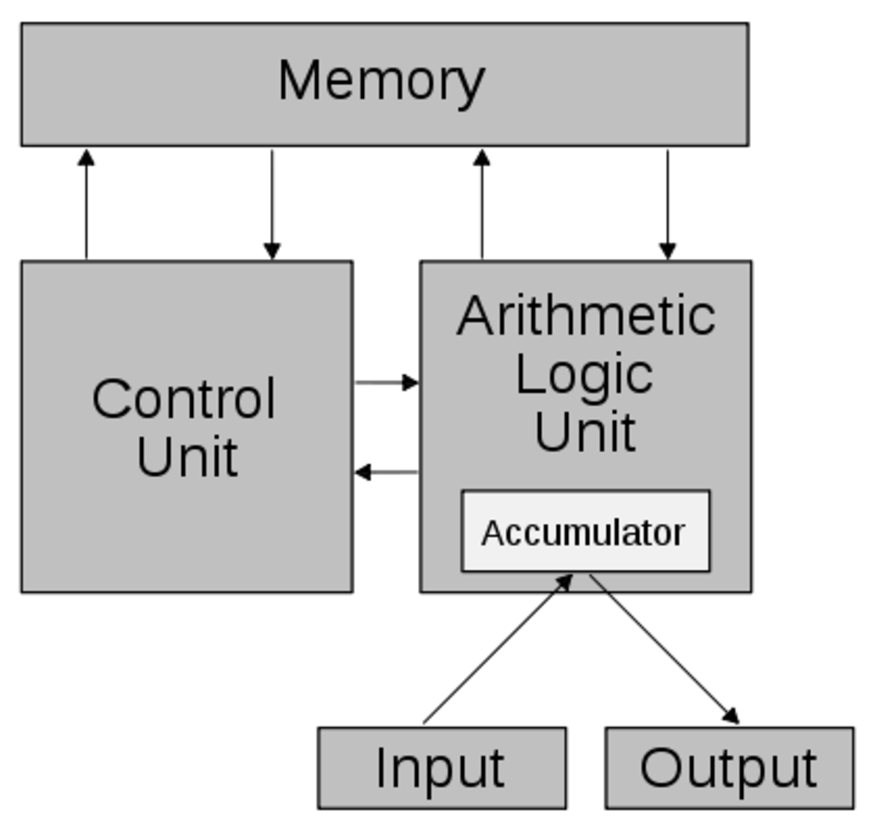
\includegraphics[width=0.5\textwidth]{figs/von-neumann.pdf}
    \end{center}
\end{frame}

%%%%%%%%%%%%%%%%%%%%%%%%%%%%%%%%%%%%
\begin{frame}{Hardware e dispositivos}
    Virtualmente todos os computadores atuais são digitais e operam com dois sinais: sem energia (0) e com energia (1)
    
    \begin{itemize}[<+->]
        \item Chamamos estes sinais de {\bf bit} $\rightarrow$ valores 0 ou 1
        \item Chamamos de {\bf byte} um agrupamento de 8 bits
        \item Todas as informações armazenadas no computador são representadas por números 0s e 1s (letras, símbolos, imagens, programas, etc.)
    \end{itemize}
\end{frame}

%%%%%%%%%%%%%%%%%%%%%%%%%%%%%%%%%%%%
\begin{frame}[fragile]{Software}

    \begin{itemize}[<+->]
        \item {\bf Softwares} são os programas que executam tarefas utilizando o hardware de um computador
        \item São compostos por um conjunto de instruções que operam o hardware
        \item Temos abaixo, por exemplo, três instruções para um computador de 32 bits
        \item Um software é composto por milhares de instruções deste tipo
        \begin{verbatim}
          0100 0010 0011 0101 0101 0100 0011 0110
          0100 1110 1100 1100 1001 0110 0110 1000
          0000 0101 1111 1110 1101 0011 0000 1100
        \end{verbatim}
    \end{itemize}
\end{frame}

%%%%%%%%%%%%%%%%%%%%%%%%%%%%%%%%%%%%
%%%%%%%%%%%%%%%%%%%%%%%%%%%%%%%%%%%%
%%%%%%%%%%%%%%%%%%%%%%%%%%%%%%%%%%%%
%%%%%%%%%%%%%%%%%%%%%%%%%%%%%%%%%%%%
%%%%%%%%%%%%%%%%%%%%%%%%%%%%%%%%%%%%
%%%%%%%%%%%%%%%%%%%%%%%%%%%%%%%%%%%%
%%%%%%%%%%%%%%%%%%%%%%%%%%%%%%%%%%%%

\section{Organização de um ambiente computacional}

%%%%%%%%%%%%%%%%%%%%%%%%%%%%%%%%%%%%%%
\begin{frame}{Organização básica de um ambiente computacional}

    \begin{center}
        \begin{tabular}{|c|} \hline
            Programas de Aplicação \\\hline
            Compiladores \\\hline
            Sistema operacional \\\hline
            Hardware \\\hline
        \end{tabular}
    \end{center}

    \begin{itemize}
        \item Um ambiente computacional é organizado como uma pilha, onde cada item da pilha realiza tarefas bem específicas
        \item Items acima na pilha fazem uso de soluções propostas pelos items abaixo
    \end{itemize}
\end{frame}

%%%%%%%%%%%%%%%%%%%%%%%%%%%%%%%%%%%%%%
\begin{frame}{Organização básica de um ambiente computacional}

    \begin{center}
        \begin{tabular}{|c|} \hline
            \textbf{Programas de Aplicação} \\\hline
            Compiladores \\\hline
            Sistema operacional \\\hline
            Hardware \\\hline
        \end{tabular}
    \end{center}

    \begin{itemize}[<+->]
        \item Como usuários, interagimos com os programas de aplicação
        \item Neste curso iremos descer nesta hierarquia, para construir novos programas de aplicação
        \item Para isso, podemos escrever diretamente códigos digitais que serão executados por um computador
        \item Mas usaremos uma linguagem de programação específica e um compilador para transformar o nosso código em um programa
    \end{itemize}
\end{frame}

%%%%%%%%%%%%%%%%%%%%%%%%%%%%%%%%%%%%%%
\begin{frame}[fragile]{Organização básica de um ambiente computacional}

    \begin{center}
        \begin{tabular}{|c|} \hline
            Programas de Aplicação \\\hline
            \textbf{Compiladores} \\\hline
            Sistema operacional \\\hline
            Hardware \\\hline
        \end{tabular}
    \end{center}

    \begin{itemize}[<+->]
        \item Um {\bf compilador} é um programa que lê um código de uma linguagem de programação e o transforma em um programa executável
        \item Ele realiza esta tarefa juntamente com um {\bf assembler}
    \end{itemize}
\end{frame}

%%%%%%%%%%%%%%%%%%%%%%%%%%%%%%%%%%%%%%
\begin{frame}[fragile]{Primeiro programa: Hello World!}

    \begin{minted}{c}
        #include <stdio.h>

        int main() {
            printf("Hello world!\n");
            return 0;
        }
    \end{minted}
\end{frame}

%%%%%%%%%%%%%%%%%%%%%%%%%%%%%%%%%%%%%%
\begin{frame}[fragile]{Primeiro programa: Hello World!}
    \begin{minted}{asm}
        global  _main
        extern  _printf
    
        section .text
    _main:
        push    message
        call    _printf
        add     esp, 4
        ret
    message:
        db  'Hello, World', 10, 0
    \end{minted}    
\end{frame}

%%%%%%%%%%%%%%%%%%%%%%%%%%%%%%%%%%%%%%
\begin{frame}[fragile]{Primeiro programa: Hello World!}
    \begin{minted}{bash}
    b8    21 0a 00 00 
    a3    0c 10 00 06 
    b8    6f 72 6c 64 
    a3    08 10 00 06 
    b8    6f 2c 20 57 
    a3    04 10 00 06 
    b8    48 65 6c 6c 
    a3    00 10 00 06 
    b9    00 10 00 06 
    ba    10 00 00 00 
    bb    01 00 00 00 
    b8    04 00 00 00 
    cd    80          
    b8    01 00 00 00 
    cd    80          
    \end{minted}
\end{frame}

%%%%%%%%%%%%%%%%%%%%%%%%%%%%%%%%%%%%%%
\begin{frame}{Organização básica de um ambiente computacional}

    \begin{center}
        \begin{tabular}{|c|} \hline
            Programas de Aplicação \\\hline
            Compiladores \\\hline
            \textbf{Sistema operacional} \\\hline
            Hardware \\\hline
        \end{tabular}
    \end{center}

    \begin{itemize}[<+->]
        \item Os programas possuem instruções que são executadas no hardware
        \item Mas o acesso ao hardware é controlado por um software especial, o \textbf{sistema operacional}
        \item Ele é o responsável pelo controle do hardware, incluindo segurança, gerenciamento de memória, dentre outros
        \item Exemplos de sistema operacionais: Windows, \textbf{Linux}, OS X, Android, iOS
    \end{itemize}
\end{frame}

\end{document}
